\chapter{Phân tích và thiết kế}

\section{Yêu cầu chức năng}

Chương trình mô phỏng điều phối tiến trình đáp ứng các yêu cầu chức năng sau:

\begin{enumerate}
    \item \textbf{Đọc dữ liệu đầu vào:} Đọc file văn bản chứa thông tin các tiến trình (thời gian đến, chuỗi CPU burst và Resource burst).
    \item \textbf{Lựa chọn thuật toán:} Hỗ trợ 4 thuật toán FCFS, RR, SJF, SRTN thông qua tham số dòng lệnh hoặc menu tương tác.
    \item \textbf{Mô phỏng theo tick:} Chạy mô phỏng từng đơn vị thời gian, cập nhật trạng thái các tiến trình, CPU và tài nguyên R.
    \item \textbf{Xuất biểu đồ Gantt:} Ghi biểu đồ Gantt của CPU và tài nguyên R ra file đầu ra.
    \item \textbf{Phân tích hiệu năng:} Tính toán và hiển thị các chỉ số response time, waiting time, turnaround time và utilization.
    \item \textbf{Chế độ TUI:} Hiển thị trực quan quá trình mô phỏng theo thời gian thực (tùy chọn).
\end{enumerate}

\section{Kiến trúc tổng thể}

Chương trình được thiết kế theo mô hình hướng đối tượng với sự phân tách trách nhiệm rõ ràng giữa các lớp. Kiến trúc tổng thể tuân theo mẫu thiết kế Strategy cho phép dễ dàng thêm mới các thuật toán điều phối.

\begin{figure}[h]
\centering
\begin{tikzpicture}[node distance=1.2cm, scale=0.6, transform shape]
\tikzstyle{io}=[rectangle, draw, fill=orange!20, minimum width=2.2cm, minimum height=0.8cm, rounded corners, align=center, font=\small]
\tikzstyle{proc}=[rectangle, draw, fill=blue!20, minimum width=2.2cm, minimum height=0.8cm, rounded corners, align=center, font=\small]
\tikzstyle{data}=[rectangle, draw, fill=green!20, minimum width=2.2cm, minimum height=0.8cm, rounded corners, align=center, font=\small]
\tikzstyle{arrow}=[->, thick]

\node[io] (input) {Input File\\ (.txt)};
\node[proc, right=1.2cm of input] (parser) {Parser};
\node[data, right=1.2cm of parser] (processes) {vector<Process>};
\node[proc, right=1.2cm of processes] (scheduler) {Scheduler};
\node[proc, below=0.8cm of scheduler] (algo) {Algorithm\\ (Strategy)};
\node[data, right=1.2cm of scheduler] (gantt) {Gantt Data};
\node[proc, right=1.2cm of gantt] (output) {Parser\\ writeOutput};
\node[io, right=1.2cm of output] (outfile) {Output File\\ (Gantt)};
\node[proc, below=0.8cm of gantt] (analytics) {Analytics};
\node[proc, below=0.8cm of scheduler] (visualizer) {Visualizer\\ (TUI)};

\draw[arrow] (input) -- (parser);
\draw[arrow] (parser) -- (processes);
\draw[arrow] (processes) -- (scheduler);
\draw[arrow] (scheduler) -- (algo);
\draw[arrow] (scheduler) -- (gantt);
\draw[arrow] (gantt) -- (output);
\draw[arrow] (output) -- (outfile);
\draw[arrow] (gantt) -- (analytics);
\draw[arrow] (scheduler) -- (visualizer);

\end{tikzpicture}
\caption{Kiến trúc tổng thể của chương trình}
\label{fig:architecture}
\end{figure}

\section{Thiết kế chi tiết các lớp}

\subsection{Lớp Process và TaskBurst}

Lớp \code{Process} biểu diễn một tiến trình trong hệ thống. Mỗi tiến trình có một danh sách các \code{TaskBurst}, mỗi burst có thể là CPU hoặc RESOURCE.

\begin{itemize}
    \item \textbf{Thuộc tính chính:} PID, arrival\_time, danh sách burst, current\_burst\_index, thời gian đáp ứng, thời gian hoàn thành, thời gian chờ.
    \item \textbf{Phương thức chính:} \code{advanceBurst()} (chuyển burst tiếp theo), \linebreak[4]\code{getRemainingCPUTotal()} (tính tổng CPU còn lại), \code{markCompletion()}, \code{markFirstResponse()}, \code{addWaitingTime()}.
\end{itemize}

\subsection{Lớp ISchedulingAlgorithm (Interface)}

Đây là interface định nghĩa phương thức \code{pickNext()} -- chiến lược chọn tiến trình tiếp theo từ hàng đợi ready. Bốn lớp con cài đặt cụ thể:

\begin{itemize}
    \item \textbf{FCFSScheduler:} Luôn chọn tiến trình ở đầu hàng đợi (index 0).
    \item \textbf{RoundRobinScheduler:} Luôn chọn index 0, preemption do Scheduler xử lý.
    \item \textbf{SJFScheduler:} Duyệt hàng đợi, chọn tiến trình có \code{getRemainingCPUTotal()} nhỏ nhất.
    \item \textbf{SRTNScheduler:} Cùng logic SJF, nhưng Scheduler gọi \code{checkSRTNPreemption()} để preempt.
\end{itemize}

\subsection{Lớp Scheduler}

\code{Scheduler} là lớp trung tâm điều phối toàn bộ quá trình mô phỏng. Nó sở hữu danh sách tiến trình, hàng đợi ready, CPU state, tài nguyên R và con trỏ tới thuật toán điều phối.

\subsection{Lớp Resource}

\code{Resource} mô hình hóa tài nguyên dùng chung R với cơ chế FCFS. Nó duy trì hàng đợi resource, tiến trình đang sử dụng, lịch sử Gantt và thời gian idle.

\subsection{Lớp Parser}

\code{Parser} là lớp tiện ích tĩnh với hai phương thức:
\begin{itemize}
    \item \code{parseInput()}: Đọc file đầu vào, phân tích cú pháp, tạo danh sách \code{Process}.
    \item \code{writeOutput()}: Ghi biểu đồ Gantt CPU và Resource ra file đầu ra.
\end{itemize}

\subsection{Lớp Visualizer}

\code{Visualizer} cung cấp giao diện TUI real-time. Mỗi tick, nó nhận \code{SystemSnapshot} (trạng thái hệ thống tại tick đó) và render lên terminal với mã màu ANSI.

\subsection{Lớp Analytics}

\code{Analytics} nhận kết quả mô phỏng, tính toán các chỉ số hiệu năng và in báo cáo dạng bảng.

\section{Class Diagram}

\begin{figure}[h]
\centering
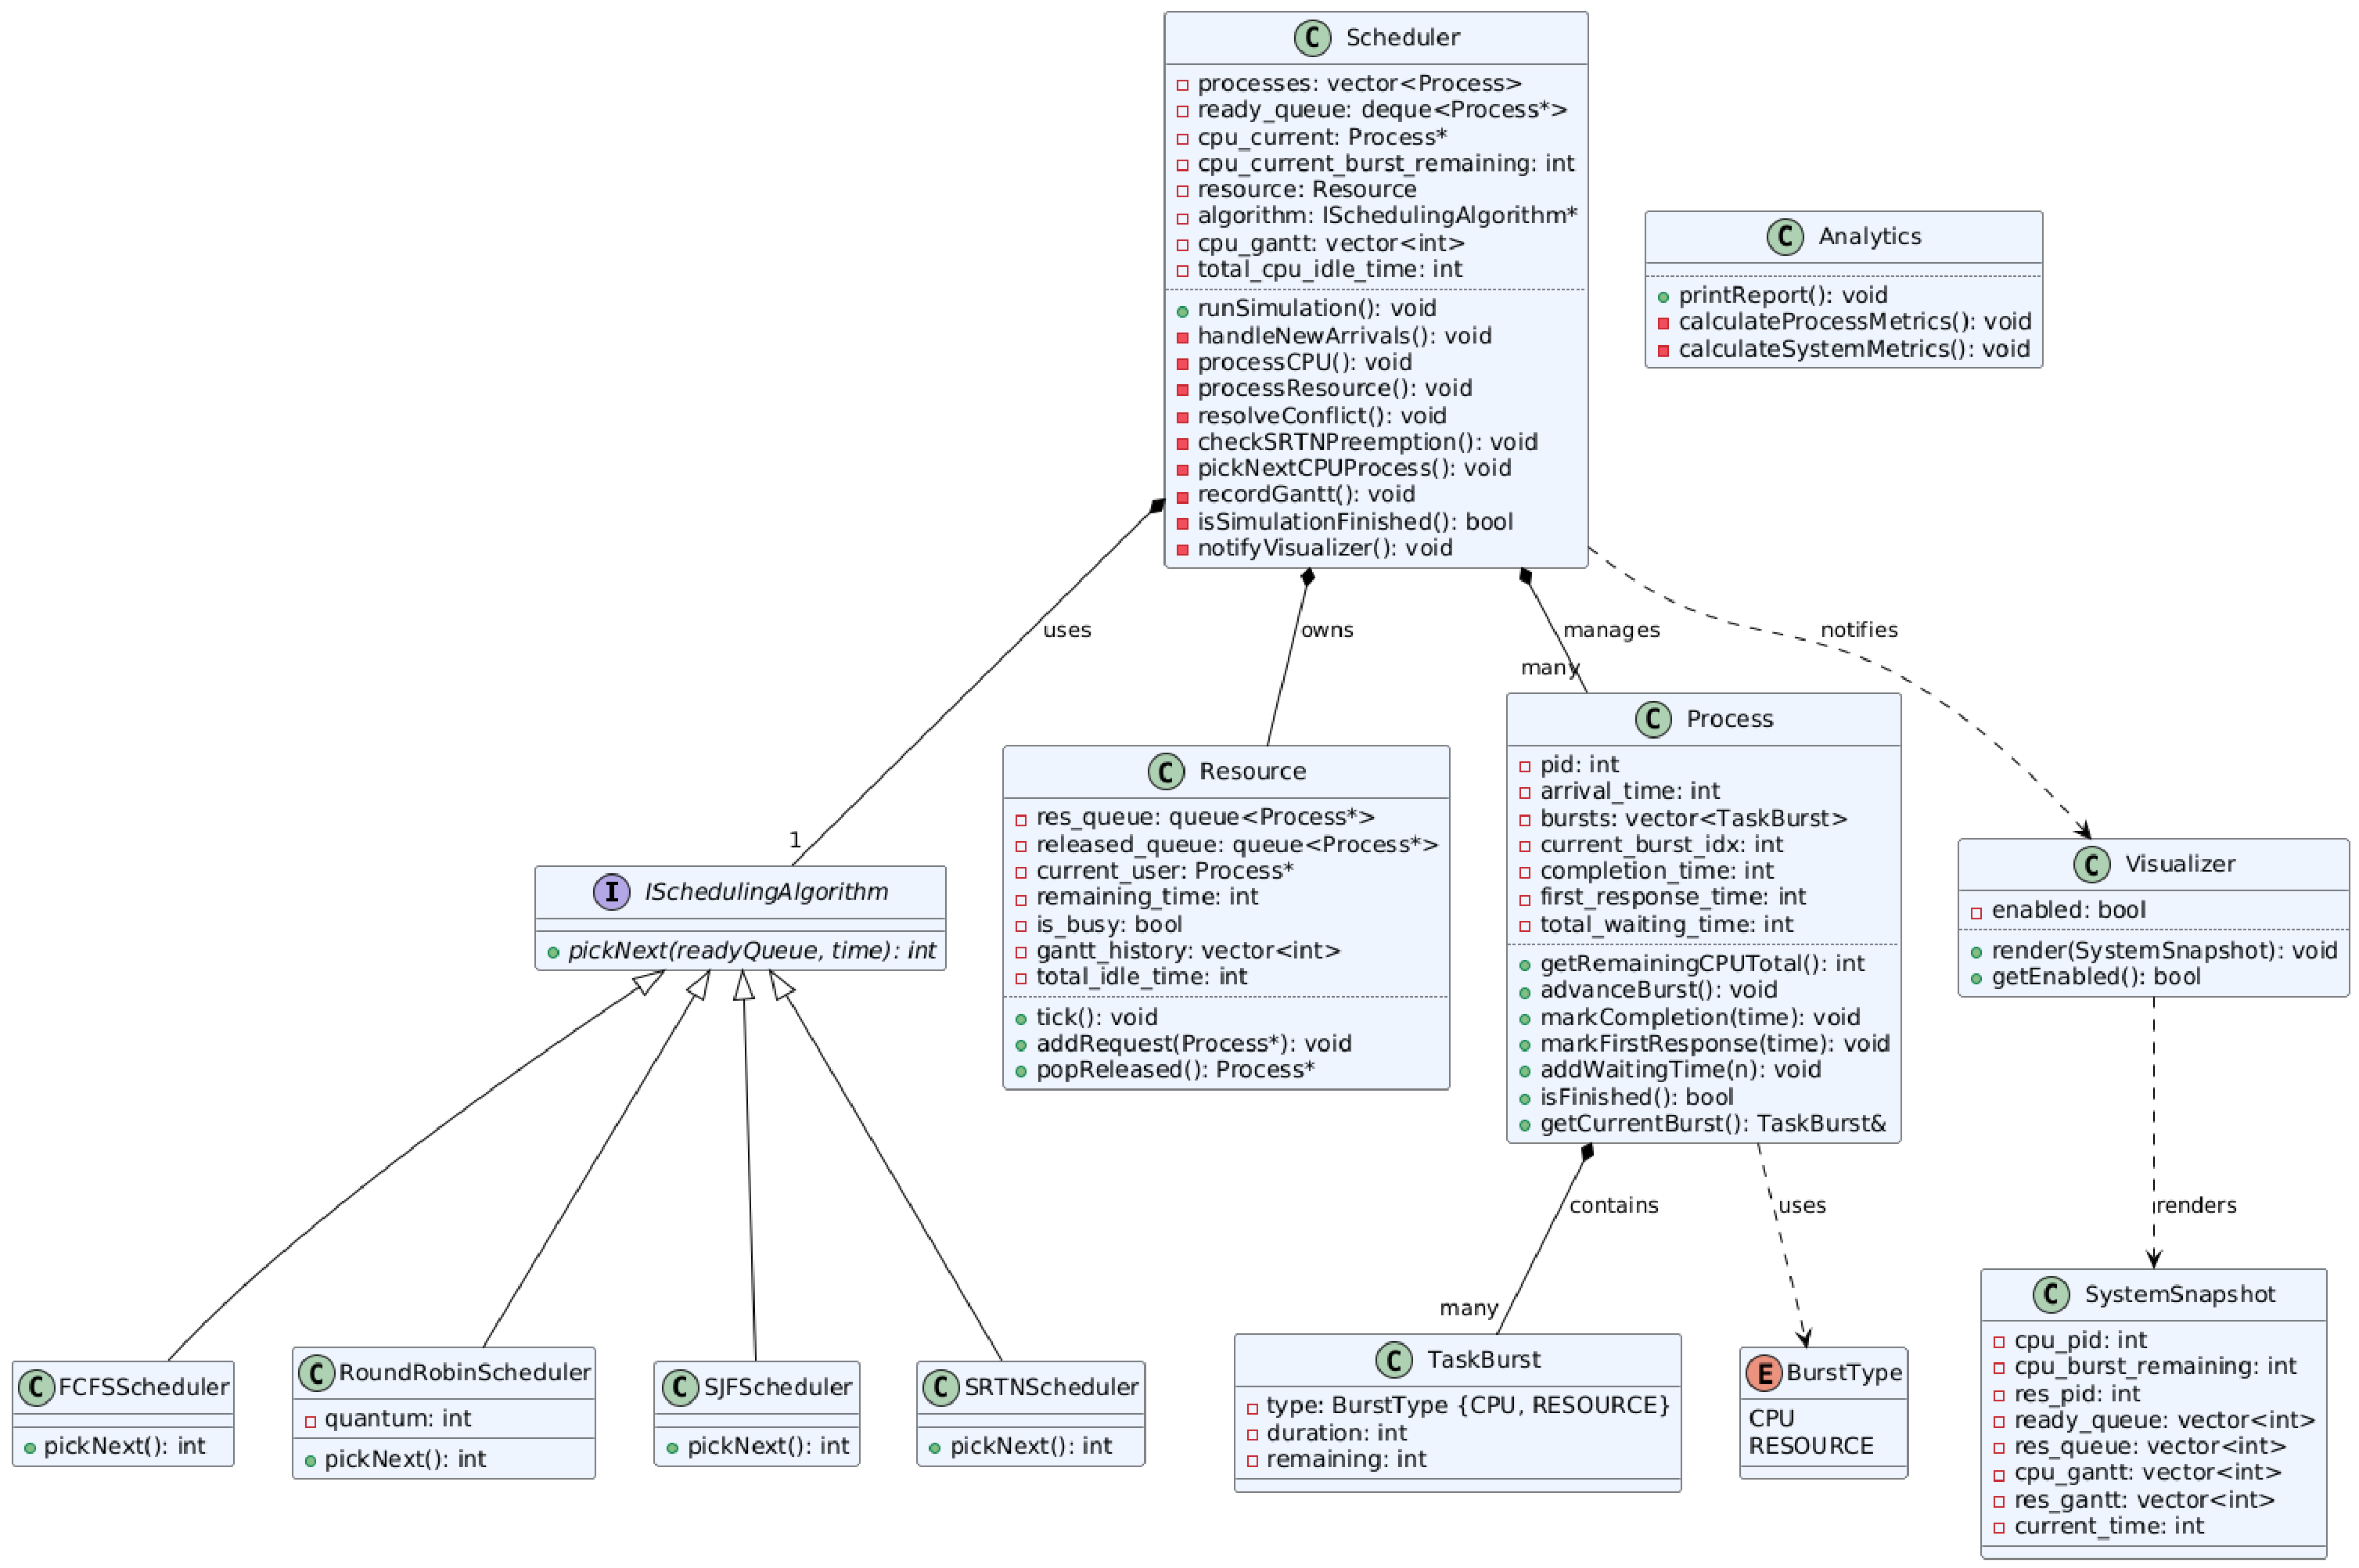
\includegraphics[width=\textwidth]{figures/class_diagram.pdf}
\caption{Class Diagram của chương trình}
\label{fig:class-diagram}
\end{figure}

\section{Sequence Diagram}

Hình~\ref{fig:sequence} mô tả luồng hoạt động chính của chương trình từ khi nhận tham số dòng lệnh đến khi xuất kết quả.

\begin{figure}[h]
\centering
\begin{tikzpicture}[node distance=0.5cm]
\tikzstyle{obj}=[rectangle, draw, minimum width=2cm, minimum height=0.7cm, rounded corners, font=\small]
\tikzstyle{line}=[thick]
\tikzstyle{arrow}=[->, thick]
\tikzstyle{return}=[<-, thick, dashed]

% Objects
\node[obj, fill=orange!20] (main) {main()};
\node[obj, right=3cm of main, fill=green!20] (parser) {:Parser};
\node[obj, right=3cm of parser, fill=blue!20] (scheduler) {:Scheduler};
\node[obj, right=3cm of scheduler, fill=red!20] (algo) {:Algorithm};

% Lifelines
\draw[line] (main.south) -- ++(0,-10cm);
\draw[line] (parser.south) -- ++(0,-10cm);
\draw[line] (scheduler.south) -- ++(0,-10cm);
\draw[line] (algo.south) -- ++(0,-10cm);

% Messages
\draw[arrow] ([yshift=-0.5cm]main.south) -- node[above, font=\tiny] {parseInput(path)} ([yshift=-0.5cm]parser.south);
\draw[return] ([yshift=-1cm]parser.south) -- node[above, font=\tiny] {vector<Process>} ([yshift=-1cm]main.south);

\draw[arrow] ([yshift=-1.8cm]main.south) -- node[above, font=\tiny] {new Scheduler(procs, algo)} ([yshift=-1.8cm]scheduler.south);

\draw[arrow] ([yshift=-2.8cm]main.south) -- node[above, font=\tiny] {runSimulation()} ([yshift=-2.8cm]scheduler.south);

% Loop box
\draw[thick, dashed] ([xshift=-2mm, yshift=-3.5cm]scheduler.south) rectangle ([xshift=2mm, yshift=-8cm]scheduler.south);
\node[font=\tiny] at ([yshift=-3.2cm]scheduler.south) {Loop per tick};

\draw[arrow] ([yshift=-4cm]scheduler.south) -- node[above, font=\tiny] {pickNext(queue)} ([yshift=-4cm]algo.south);
\draw[return] ([yshift=-4.5cm]algo.south) -- node[above, font=\tiny] {int idx} ([yshift=-4.5cm]scheduler.south);

\node[font=\tiny] at ([yshift=-6.5cm]scheduler.south) {Process CPU / Resource};

\draw[arrow] ([yshift=-9cm]main.south) -- node[above, font=\tiny] {writeOutput()} ([yshift=-9cm]parser.south);

\end{tikzpicture}
\caption{Sequence Diagram luồng chính}
\label{fig:sequence}
\end{figure}

\section{Cấu trúc dữ liệu}

\subsection{Hàng đợi Ready (Ready Queue)}

Hàng đợi ready được cài đặt bằng \code{std::deque<Process*>} (double-ended queue). Hàng đợi này hỗ trợ thêm phần tử ở cuối (khi tiến trình vào ready) và lấy phần tử ở đầu (khi CPU pick next process). Khi có xung đột (nhiều tiến trình vào ready cùng lúc), tiến trình mới đến được ưu tiên trước tiến trình trả về từ Resource R.

\subsection{Hàng đợi Resource}

Tài nguyên R duy trì hai hàng đợi \code{std::queue<Process*>}:
\begin{itemize}
    \item \textbf{res\_queue:} Hàng đợi FCFS các tiến trình đang chờ tài nguyên R.
    \item \textbf{released\_queue:} Hàng đợi các tiến trình vừa hoàn thành Resource burst, chờ được đưa trở lại ready queue.
\end{itemize}

\subsection{Hệ thống Snapshot cho TUI}

Cấu trúc \code{SystemSnapshot} được truyền từ \code{Scheduler} đến \code{Visualizer} mỗi tick, chứa toàn bộ trạng thái hiện tại:
\begin{itemize}
    \item Tiến trình đang chạy trên CPU (PID + burst còn lại).
    \item Tiến trình đang sử dụng Resource R.
    \item Danh sách các tiến trình trong ready queue.
    \item Danh sách các tiến trình trong resource queue.
    \item Lịch sử Gantt đã ghi nhận.
\end{itemize}
